%%%%%%%%%%%%%%%%%%%%%%%%%%%%%%%%%%%%%%%%%
% Arsclassica Article
% LaTeX Template
% Version 1.1 (10/6/14)
%
% This template has been downloaded from:
% http://www.LaTeXTemplates.com
%
% Original author:
% Lorenzo Pantieri (http://www.lorenzopantieri.net) with extensive modifications by:
% Vel (vel@latextemplates.com)
%
% License:
% CC BY-NC-SA 3.0 (http://creativecommons.org/licenses/by-nc-sa/3.0/)
%
%%%%%%%%%%%%%%%%%%%%%%%%%%%%%%%%%%%%%%%%%

%----------------------------------------------------------------------------------------
%	PACKAGES AND OTHER DOCUMENT CONFIGURATIONS
%----------------------------------------------------------------------------------------

\documentclass[
	12pt, % Main document font size
	a4paper, % Paper type, use 'letterpaper' for US Letter paper
	oneside, % One page layout (no page indentation)
	%twoside, % Two page layout (page indentation for binding and different headers)
	headinclude,footinclude, % Extra spacing for the header and footer
	BCOR5mm, % Binding correction
]{scrartcl}

%%%%%%%%%%%%%%%%%%%%%%%%%%%%%%%%%%%%%%%%%
% Arsclassica Article
% Structure Specification File
%
% This file has been downloaded from:
% http://www.LaTeXTemplates.com
%
% Original author:
% Lorenzo Pantieri (http://www.lorenzopantieri.net) with extensive modifications by:
% Vel (vel@latextemplates.com)
%
% License:
% CC BY-NC-SA 3.0 (http://creativecommons.org/licenses/by-nc-sa/3.0/)
%
%%%%%%%%%%%%%%%%%%%%%%%%%%%%%%%%%%%%%%%%%

%----------------------------------------------------------------------------------------
%	REQUIRED PACKAGES
%----------------------------------------------------------------------------------------

\usepackage[
nochapters, % Turn off chapters since this is an article        
beramono, % Use the Bera Mono font for monospaced text (\texttt)
eulermath,% Use the Euler font for mathematics
pdfspacing, % Makes use of pdftex’ letter spacing capabilities via the microtype package
dottedtoc % Dotted lines leading to the page numbers in the table of contents
]{classicthesis} % The layout is based on the Classic Thesis style

\usepackage{arsclassica} % Modifies the Classic Thesis package

\usepackage[T1]{fontenc} % Use 8-bit encoding that has 256 glyphs

\usepackage[utf8]{inputenc} % Required for including letters with accents

\usepackage{graphicx} % Required for including images
\graphicspath{{Figures/}} % Set the default folder for images

\usepackage{enumitem} % Required for manipulating the whitespace between and within lists

\usepackage{lipsum} % Used for inserting dummy 'Lorem ipsum' text into the template

\usepackage{subfig} % Required for creating figures with multiple parts (subfigures)

\usepackage{amsmath,amssymb,amsthm} % For including math equations, theorems, symbols, etc

\usepackage{varioref} % More descriptive referencing

%----------------------------------------------------------------------------------------
%	THEOREM STYLES
%---------------------------------------------------------------------------------------

\theoremstyle{definition} % Define theorem styles here based on the definition style (used for definitions and examples)
\newtheorem{definition}{Definition}

\theoremstyle{plain} % Define theorem styles here based on the plain style (used for theorems, lemmas, propositions)
\newtheorem{theorem}{Theorem}

\theoremstyle{remark} % Define theorem styles here based on the remark style (used for remarks and notes)

%----------------------------------------------------------------------------------------
%	HYPERLINKS
%---------------------------------------------------------------------------------------

\hypersetup{
%draft, % Uncomment to remove all links (useful for printing in black and white)
colorlinks=true, breaklinks=true, bookmarks=true,bookmarksnumbered,
urlcolor=webbrown, linkcolor=RoyalBlue, citecolor=webgreen, % Link colors
pdftitle={}, % PDF title
pdfauthor={\textcopyright}, % PDF Author
pdfsubject={}, % PDF Subject
pdfkeywords={}, % PDF Keywords
pdfcreator={pdfLaTeX}, % PDF Creator
pdfproducer={LaTeX with hyperref and ClassicThesis} % PDF producer
} % Include the structure.tex file which specified the document structure and layout

\hyphenation{Fortran hy-phen-ation} % Specify custom hyphenation points in words with dashes where you would like hyphenation to occur, or alternatively, don't put any dashes in a word to stop hyphenation altogether

%----------------------------------------------------------------------------------------
%	TITLE AND AUTHOR(S)
%----------------------------------------------------------------------------------------

\title{\normalfont\spacedallcaps{Generazione delle categorie di wikipedia attraverso il clustering}} % The article title

\author{\spacedlowsmallcaps{Cazzaro Dalla Cia Lovisotto Vianello}}

\date{} % An optional date to appear under the author(s)

%----------------------------------------------------------------------------------------

\begin{document}

%----------------------------------------------------------------------------------------
%	HEADERS
%----------------------------------------------------------------------------------------

\renewcommand{\sectionmark}[1]{\markright{\spacedlowsmallcaps{#1}}} % The header for all pages (oneside) or for even pages (twoside)
%\renewcommand{\subsectionmark}[1]{\markright{\thesubsection~#1}} % Uncomment when using the twoside option - this modifies the header on odd pages
\lehead{\mbox{\llap{\small\thepage\kern1em\color{halfgray} \vline}\color{halfgray}\hspace{0.5em}\rightmark\hfil}} % The header style

\pagestyle{scrheadings} % Enable the headers specified in this block

%----------------------------------------------------------------------------------------
%	TABLE OF CONTENTS & LISTS OF FIGURES AND TABLES
%----------------------------------------------------------------------------------------

\maketitle % Print the title/author/date block

\newpage

%----------------------------------------------------------------------------------------
%	INTRODUCTION
%----------------------------------------------------------------------------------------

\section{Introduzione}

Per il progetto del corso di Data Mining abbiamo deciso di svolgere la traccia proposta B, che proponeva di indagare fino a che punto un clustering sulle pagine di Wikipedia è consistente con le categorie associate alle pagine tesse.
Per fare ciò avevamo a disposizione due dataset, di differenti grandezze, formati da articoli di Wikipedia in lingua inglese.

A partire da tali premesse ci siamo prefissati i seguenti quesiti:

\begin{itemize}
	\item quanto sono clusterizzabili gli articoli del dataset?
	\item le categorie associate a questi articoli sono sensate?
	\item quali sono dei metodi validi per rappresentare opportunamente i nostri dati in input?
	\item come variano i cluster utilizzando tecniche diverse?
	\item c'è un numero ottimale di cluster per il dataset? Quanto vale?
	\item qual è il rapporto tra il cluster ottenuto e le categorie?
\end{itemize}

Tali quesiti troveranno risposta nel seguito della trattazione, che è strutturata nel modo che segue.
La sezione 2 illustra l'analisi preliminare effettuata sugli articoli e sulle categorie.
Successivamente il capitolo 3 descrive le tecniche utilizzate per rappresentare il dataset.
Il capitolo 4 tratta poi degli algoritmi di clustering applicati al dataset e delle tecniche di valutazione impiegate.
Di seguito la sezione 5 riporta e discute i risultati ottenuti nel capitolo precedente, offrendo anche un confronto tra i metodi utilizzati.
Infine la sezione 6 riassume il lavoro svolto, ciò che abbiamo ottenuto e propone alcuni spunti di ricerca per futuri sviluppi.


\section{Dataset e Analisi Preliminare}
	Ci sono stati messi a disposizione due dataset, di differenti grandezze, per effettuare questa analisi.
	Nello specifico abbiamo utilizzato quello minore, il quale è un \emph{dump} composto da un JSON contenente centomila articoli di Wikipedia in versione inglese.
	Per ogni articolo abbiamo a disposizione il titolo, il testo, l'id e le categorie dell'articolo.
	In particolare le categorie sono assegnate a discrezione degli autori e dei successivi revisori di ogni voce, in quanto Wikipedia non prevede una struttura o dei vincoli particolari per l'assegnazione di queste categorie.

	La nostra analisi mira a valutare la relazione semantica tra gli articoli e le loro categorie, quindi prima di effettuare l'analisi si è deciso di eliminare tutti gli articoli che non risultano essere associati a nessuna categoria. Queste pagine sono dette \emph{di disambiguazione} e quindi non sono utili per i nostri scopi.

	Per quanto concerne le categorie, una prima ispezione manuale rivela che esse sono alquanto arbitrarie e spesso così specifiche da essere associate ad un articolo soltanto.
	Esempio di ciò sono le categorie "Roads on the National Register of Historic Places in Illinois", "United Nations Security Council resolutions concerning Sudan" e "Singaporean people of Yemeni descent".
    C'è inoltre da sottolineare come ad ogni articolo siano spesso associate più di una categoria, con una media di 1.99 categorie per ogni voce del dataset.
    
    Un'analisi più approfondita sulla distribuzione delle categorie è riportata in figura \ref{fig:categories}. 
    \begin{figure}[!htb]
			\centering
			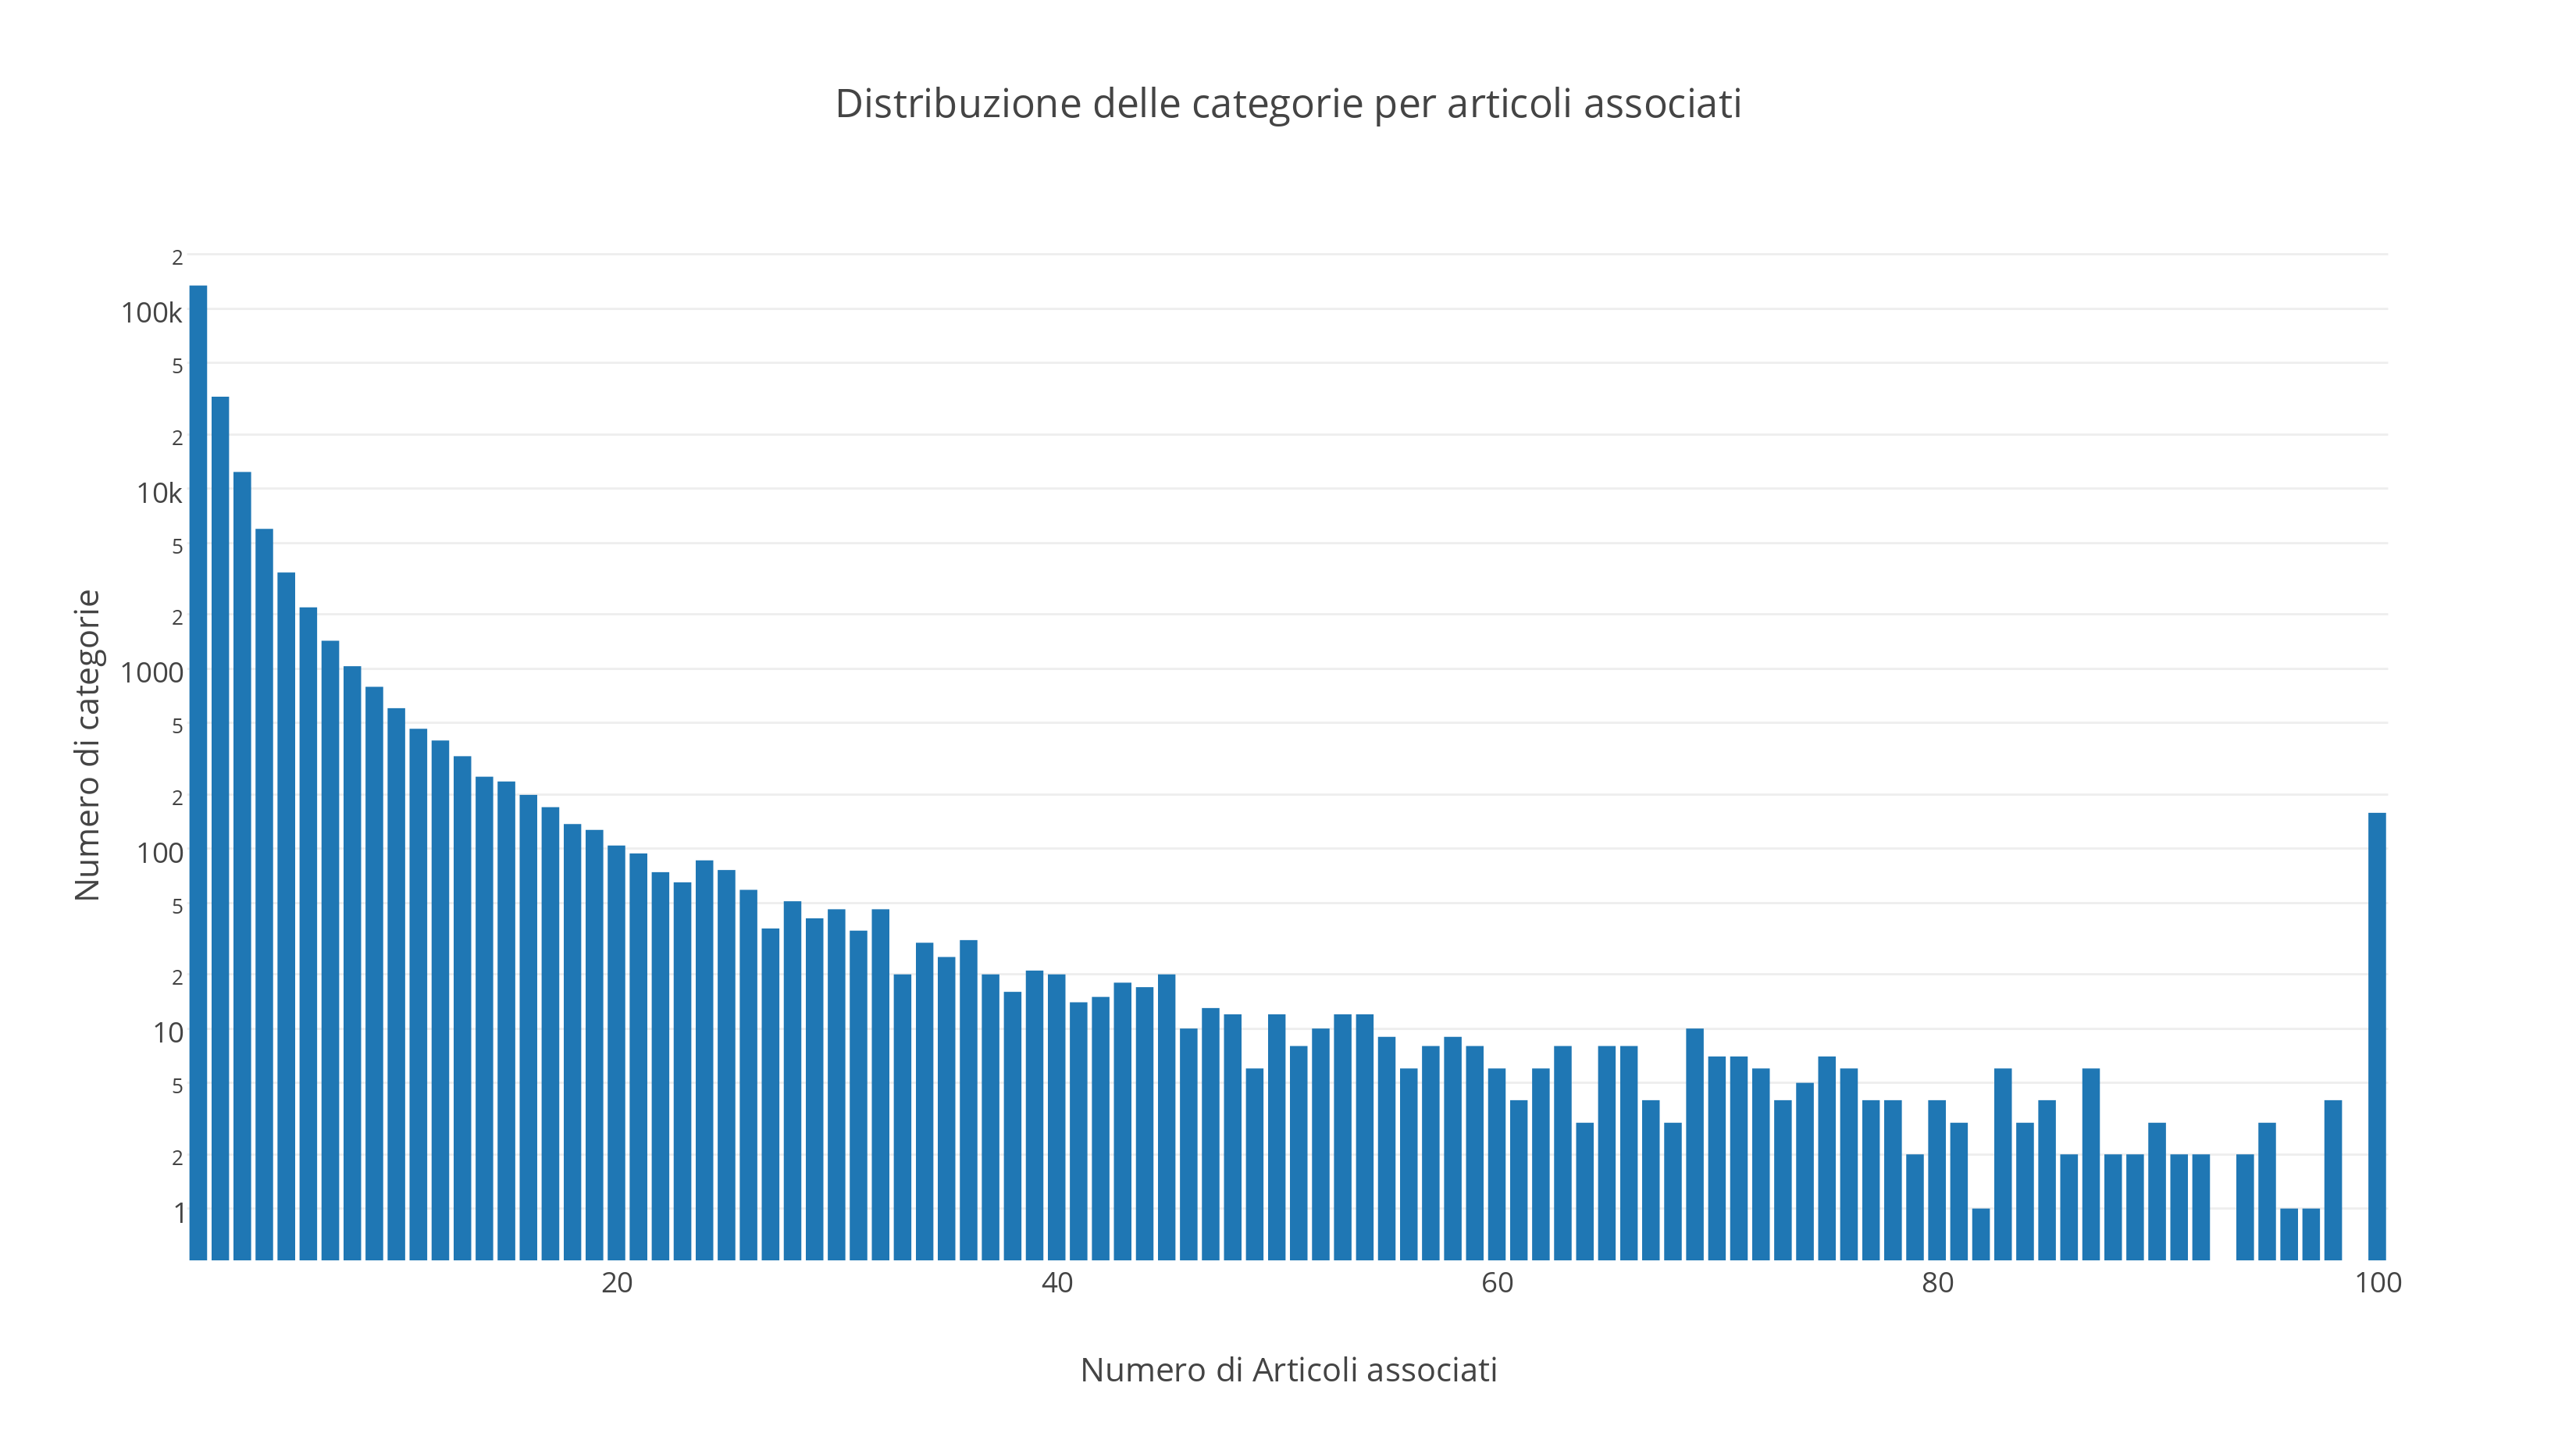
\includegraphics[scale=.5]{Figures/categories.png}
			\caption{Distribuzione delle categorie. Nota: per rendere il grafico leggibile il picco finale raggruppa il numero di categorie con cento o più articoli.}
			\label{fig:categories}
		\end{figure}
   
	L'analisi effettuata rivela infatti che, sul totale di 198609 distinte categorie presenti nel dataset, circa due terzi (precisamente 134524) di queste sono uniche, ovvero sono associate ad un solo articolo.
	Dato che queste non portano alcun contenuto informativo utile alla clusterizzazione, abbiamo provveduto ad escludere tali categorie dalle successive analisi.

	Nondimeno è anche presente un numero ristretto di 158 categorie associate a 100 o più articoli, le quali sono composte per lo più da categorie del genere "1900 deaths" e "1900 births" che si ripetono variando solamente l'anno.
	In tabella \ref{table:toptencategories} sono riportate a titolo di esempio le categorie con più articoli associati.


	\begin{table}[]
	\centering
	\caption{Le categorie con maggior numero di articoli associati}
	\label{table:toptencategories}
	\begin{tabular}{l|l|l|l|l}
	Living people & 14994 & Association football midfielders & 611 \\
	Year of birth missing (living people) & 1172 & Association football defenders & 502 \\
	Place of birth missing (living people) & 751 & Association football forwards & 409 \\
	American films & 741 & Year of birth unknown & 404 \\
	English-language films & 691 & English Football League players & 398 \\
	\end{tabular}
	\end{table}



\section{Rappresentazione del Dataset}
	Prima di procedere con qualsiasi operazione sull'intero corpus si è deciso di preprocessare il data set eliminando le cosiddette \emph{stop words} presenti nel testo e lemmatizzando le parole rimaste.
	
	Per l'eliminazione delle \emph{stop words} ci siamo basati su una lista di parole fornita dal sito http://www.ranks.nl/stopwords. 
	Questi termini vengono filtrati dal corpus in quanto portano un contenuto informativo sull'argomento dell'articolo pressoch\'{e} nullo.
	
	La lemmatizzazione invece \'{e} stata eseguita utilizzando il $Lemmatizer$ di spark al fine di raggruppare assieme le variazioni semantiche delle parole.
	
	\subsection{VETTORIALIZZIONE DEGLI ARTICOLI}

        Per interagire con i più comuni algoritmi di clustering, ad esempio K-means, si è reso necessario trasformare
        gli articoli di Wikipedia in vettori.
        Per fare ciò abbiamo adottato una tecnica nota in letteratura con il nome Word2Vec. Tale algoritmo ideato da
        Tomas Mikolov non è altro che una rete neurale a due strati il cui scopo è quello di trasformare parole del
        linguaggio naturale in vettori. Nello spazio vettoriale generato le parole semanticamente più simili
        saranno più vicine, viceversa parole semanticamente diverse risulteranno distanti.

        Tale funzionalità è già implementata nella suite software di Spark,
        per sfruttarla è necessario inizializzare alcuni parametri di settaggio. Tra questi uno dei più importanti
        è sicuramente la dimensione del vettore in uscita. In letteratura si è valutato che una dimensionalità
        nel ordine dei 100/300 \cite{w2vdim}
        è sufficiente a rappresenta un buon compromesso in termini di performance.
        Uno volta settati i parametri l'algoritmo di Word2Vec necessita di essere allenato. Tale allenamento è stato
        fatto su tutto il corpus.

        Per trasformare un articolo è stato sufficiente effettuare la media vettoriale di tutte le parole presenti
        nel testo di un'articolo. Tale operazione è stata eseguita attraverso il BLAS (Basic Linear Algebra Subprograms)
        di Spark per eseguire tali conti nella maniera più efficiente possibile.


	\subsection{BAG OF WORDS}

	L'algoritmo Bag of Words\cite{bagofwords} effettua la conversione degli articoli in vettori considerando le occorrenze dei termini in essi.
	In particolare viene considerata come metrica la \textit{Term frequency-inverse document frequency} (Tf-Idf).
	
	Si definisce la Tf-Idf relativa all'$i$-esimo termine nel $j$-esimo articolo come:
	$$
	w_{i,j}=tf_{i,j}\times\log(\frac{N}{df_{i}})
	$$
	dove $tf_{i,j}$ rappresenta il numero di occorrenze di $i$ in $j$, $df_{i}$ \`{e} il numero di documenti contenenti il termine $i$, ed $N$ \`{e} il numero totale di documenti.
	
	Abbiamo scelto di limitare l'analisi alle 3000 parole pi\`{u} frequenti nel dataset (escludendo le stopwords).
	
	Pertanto il modello prodotto associa ad ogni documento un vettore di dimensione 3000, contenente gli indici TfIdf associati ad ogni articolo per tutte le parole selezionate.
	


\section{Clustering}

	\subsection{Tecniche di Clustering}

		\subsubsection{Hopkins Statistic}
			Riportiamo lo score che ci dice che il nostro dataset è ben clusterizzabile

		\subsubsection{Kmeans}
			Kmeans e il suo score con un bel grafico

		\subsubsection{Altri metodi}

			Abbiamo provato anche il clustering gerarchico e il Gaussian Mixture Model
			ma non abbiamo abbastanza potenza di calcolo

		\subsubsection{Latent Dirichlet Allocation}

			Vediamo cosa viene fuori e un bel grafico


	\subsection{Valutazioni del Clustering}

		\subsubsection{Simple Silhouette}
			Utilizzo della versione semplificata di Silhouette con i centroidi
			Rimozione dei cluster con un solo articolo dal punteggio
			Magari buttiamoci un peso a sta metrica

		\subsubsection{Normalized Mutual Information}
			L'informazione mutua è una quantità che misura la mutua dipendenza di due variabili aleatorie, ovvero quanta informazione porta sull'altra la conoscenza del valore di una delle due.

			Questa misura può essere impiegata per valutare quanto due partizioni, o \emph{clustering}, concordano nel suddividere un set di punti \cite{Manning}.

			Per fare questo, ad ogni cluster è stata associata una variabile indicatrice $\omega$, che assume valore 1 se il punto considerato appartiene al cluster e 0 altrimenti.
			Ogni clustering viene perciò individuato dall'insieme $\Omega$ di queste variabili aleatorie mutualmente esclusive e a somma unitaria.

			Con questa descrizione del problema è possibile calcolare l'informazione mutua tra due distinti clustering $\Omega$ e $\Phi$.
			Questa matrica è stata normalizzata in $(0, 1)$ per garantire un confronto alla pari tra clustering di dimensione diversa.

			NMI viene quindi definita come
			\begin{equation} \begin{aligned} \label{eq:NMI}
				& NMI(\Omega, \Phi) = \frac
					{I(\Omega, \Phi)}
					{\left[ H(\Omega) + H(\Phi)\right] / 2} \\
				& \text{dove} \\
				& I(\Omega, \Phi) =
					\sum_{\omega \in \Omega} \sum_{\phi \in \Phi}
						P(\omega \cap \phi) \log \frac {P(\omega \cap \phi)} {P(\omega) P(\phi)} \\
				& H(\Omega) = - \sum_{\omega \in \Omega} P(\omega) \log P(\omega) \\
				& H(\Phi) = - \sum_{\phi \in \Phi} P(\phi) \log P(\phi) \\
			\end{aligned} \end{equation}

			All'atto pratico, come valore delle probabilità sono stati impegate stime a massima verosimiglianza, per esempio
			\begin{equation*}
				P(\omega) = \frac
					{ \text{numero di punti in }\omega }
					{ \text{numero di punti totali} }
			\end{equation*}.

			\bigbreak

			Purtroppo questa definizione non è direttamente applicabile al confronto tra cluster e categorie perché, mentre i clustering ottenuti con K-means e LDA sono delle effettive partizioni del dataset, non si può dire lo stesso delle categorie, dato che un articolo può possederne più di una.

			% TODO link o descrizione della IDF utilizzata
			Il primo approccio per scogliere questo nodo è stato quello di eseguire un \emph{ranking} con \emph{Inverse Document Frequency} tra le categorie di ciascun articolo per eleggere la più rappresentativa.
			Grazie a questo passaggio NMI viene calcolata come dalla sua definizione (equazione \ref{eq:NMI}).

			% TODO specificare meglio la normalizzazione
			Il secondo approccio tenta invece di estendere NMI al caso di cluster che si sovrappongano l'uno all'altro, considerando quindi ogni classe $c$ con la sua complementare $\bar{c}$ una partizione dell'insieme dei punti.
			L'informazione mutua viene calcolata quindi per ogni clustering $C = \{c, \bar{c}\}$ e si valuta la loro somma. A causa di questa passaggio si perde la normalizzazione tra 0 e 1: i risultati sono comunque confrontabili, perché risultano tutti multipli di un fattore che è funzione della distribuzione delle categoerie, quindi indipendente dalle  tecniche di clustering.

\section{Risultati}

	\subsection{Numero di cluster}
		Il clustering K-means risulta il più semplice e rapido da ottenere e per questo motivo abbiamo deciso di ispezionare un ampio range di valori per K, numero di cluster.
		
		La funzione obiettivo cala continuamente al variare del numero di cluster, come da figura \ref{fig:KMeansObj}: questa osservazione è confermata dall'andamento della derivata della funzione obiettivo rispetto a K. Essa raggiunge un tasso di incremento trascurabile in prossimità del valore K=100.
		
		Perciò con la tecnica di clustering LDA ci siamo concentrati su valori di K compresi tra 50 e 150.
		
		\begin{figure}[!htb]
			\hspace{-2cm}
			\begin{subfigure}{.5\textwidth}
				\centering
				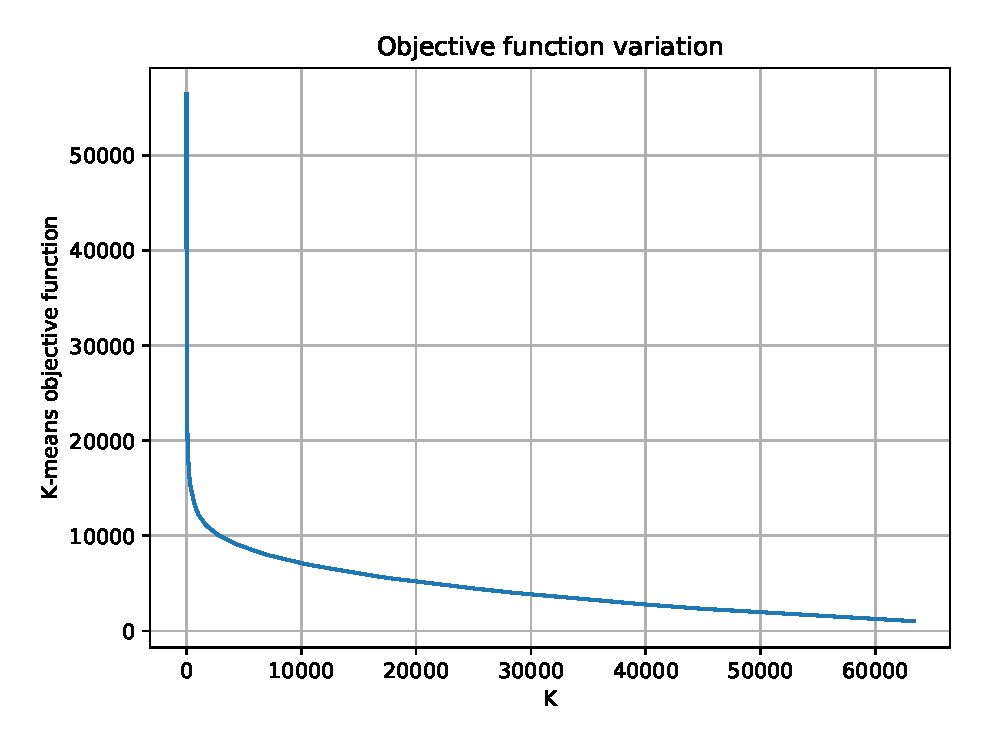
\includegraphics[scale=.5]{../results/KMeans.eps}
				\caption{Funzione obiettivo}
			\end{subfigure}
			\hspace{1.5cm}
			\begin{subfigure}{.5\textwidth}
				\centering
				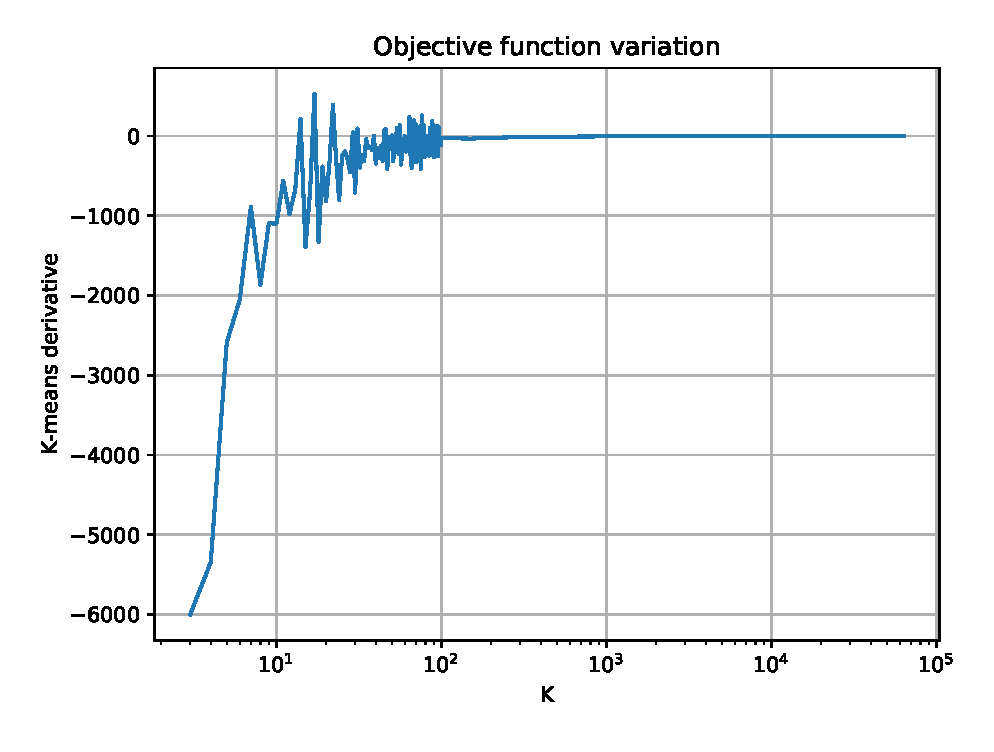
\includegraphics[scale=.5]{../results/KMeansDerivative.eps}
				\caption{Derivata della funzione obiettivo}
			\end{subfigure}
			\caption{La funzione obiettivo smette di calare in modo significativo tra 50 e 150.}
			\label{fig:KMeansObj}
		\end{figure}

	\subsection{Validazione con Simple Silhouette}
		\begin{figure}[!htb]
			\centering
			
\includegraphics[scale=.5]{../results/silhouette.eps}
			\caption{Silhouette}
			\label{fig:silhouette}
		\end{figure}
		
	\subsection{Confronto tra i Cluster ottenuti con Normalize Mutual Information}
		\begin{figure}[!htb]
			\centering
			%TODO: dava un errore..
			%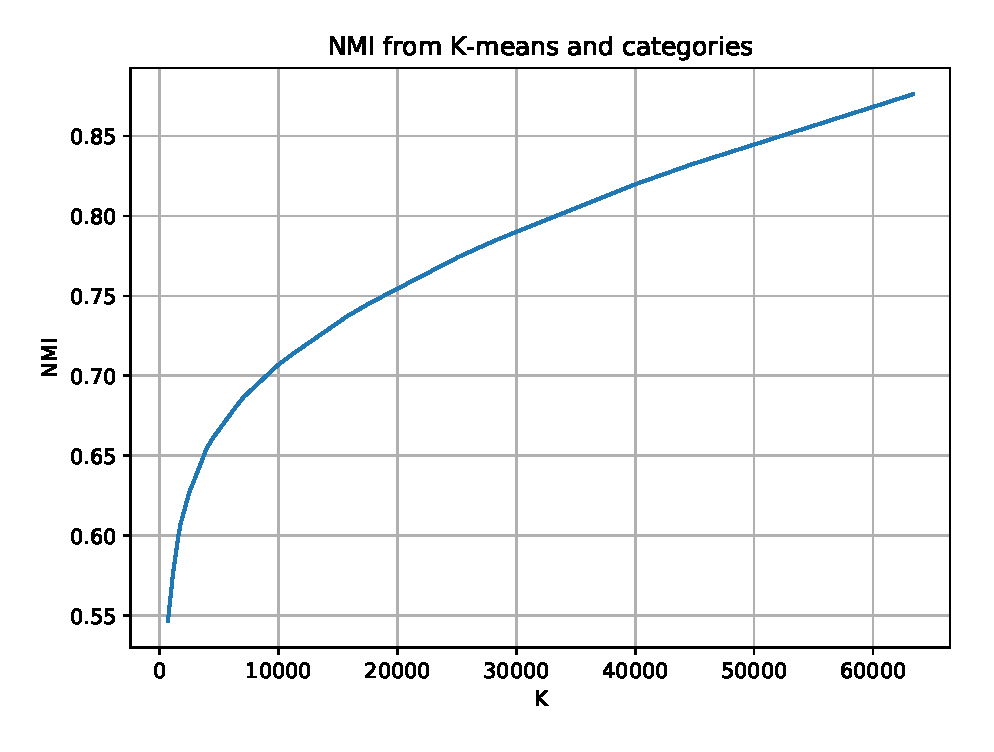
\includegraphics[scale=.5]{../results/NMI-kmeans-categories.eps}
			\caption{Informazione mutua tra K-means e il clustering indotto dalle categorie.}
			\label{fig:NMI-kmeans-categories}
		\end{figure}
		
\section{Conclusioni}
	Le conclusioni generali dalle analisi effettuate
	Proposte di punti da approfondire in studi futuri

%------------------------------------------------------------------------------
%	BIBLIOGRAPHY
%------------------------------------------------------------------------------

\begin{thebibliography}{12}

\bibitem{w2vdim}
    Tomas Mikolov, Kai Chen, Greg Corrado, and Jeffrey Dean. Efficient estimation of word representations
    in vector space. ICLR Workshop, 2013.

\bibitem{Manning}
	Christopher D. Manning, Prabhakar Raghavan and Hinrich Schütze, Introduction to Information Retrieval, Cambridge University Press. 2008

\bibitem{bagofwords}
	Harris, Zellig S. "Distributional structure." Word 10.2-3 (1954): 146-162.
	
\bibitem{lda}
	Blei, David M., Andrew Y. Ng, and Michael I. Jordan. "Latent dirichlet allocation." Journal of machine Learning research 3.Jan (2003): 993-1022.
	
\end{thebibliography}

%----------------------------------------------------------------------------------------

\end{document}
